\startchapter{Making Socio Technical Congruence Actionable}
\label{chap:actionable}
This Chapter concludes the work of this thesis by exploring the final research question \textbf{RQ 2.4:} \emph{Can recommendations be given in a timely manner?}
To explore this final question we first present how such a recommender system might look like to motivate its potential usefulness and continue with describing our study in a student course setting to answer our final research question.

\section{Recommender System: Chat To Succeed}
Most software projects have infrastructure in place that automatically builds the software system on a regular basis. 
If there are errors in this build, if automated regression tests fail, or if a developer finds a major flaw in a build this build is considered as a failed build.  
Research shows that communication structures can be used to predict the outcome of a build~\cite{wolf:icse:2009}.  
Certain patterns of communication among team members who contribute to the code can determine if a build fails or succeeds. 
We expand this idea by providing specific recommendations of who should chat together to ensure a successful build.

We showed in Chapter~\ref{} evidence that a build might fail due to a possibility that members of the software team coordinated poorly between the time the current build broke, and the last known successful build. 
One possible reason for this lack of coordination is that the team members who worked on interrelated components failed to inform each other about their changes. 
This brings us to the discussion of socio-technical congruence.

\subsection{Socio-technical Gaps}
Socio-technical congruence defines the match of technical and social dependencies among people, for example tasks (technical) and task related communication (social)~\cite{cataldo:cscw:2006}. 
It compares a technical network to a communication network and identifies gaps where a coordination need exists, but no communication fills the gap. 
We showed that gaps have a negative influence on the project~\cite{} as well as that there are specific gaps that correlate to build failure~\cite{}. 

\begin{figure}[t]
\centering
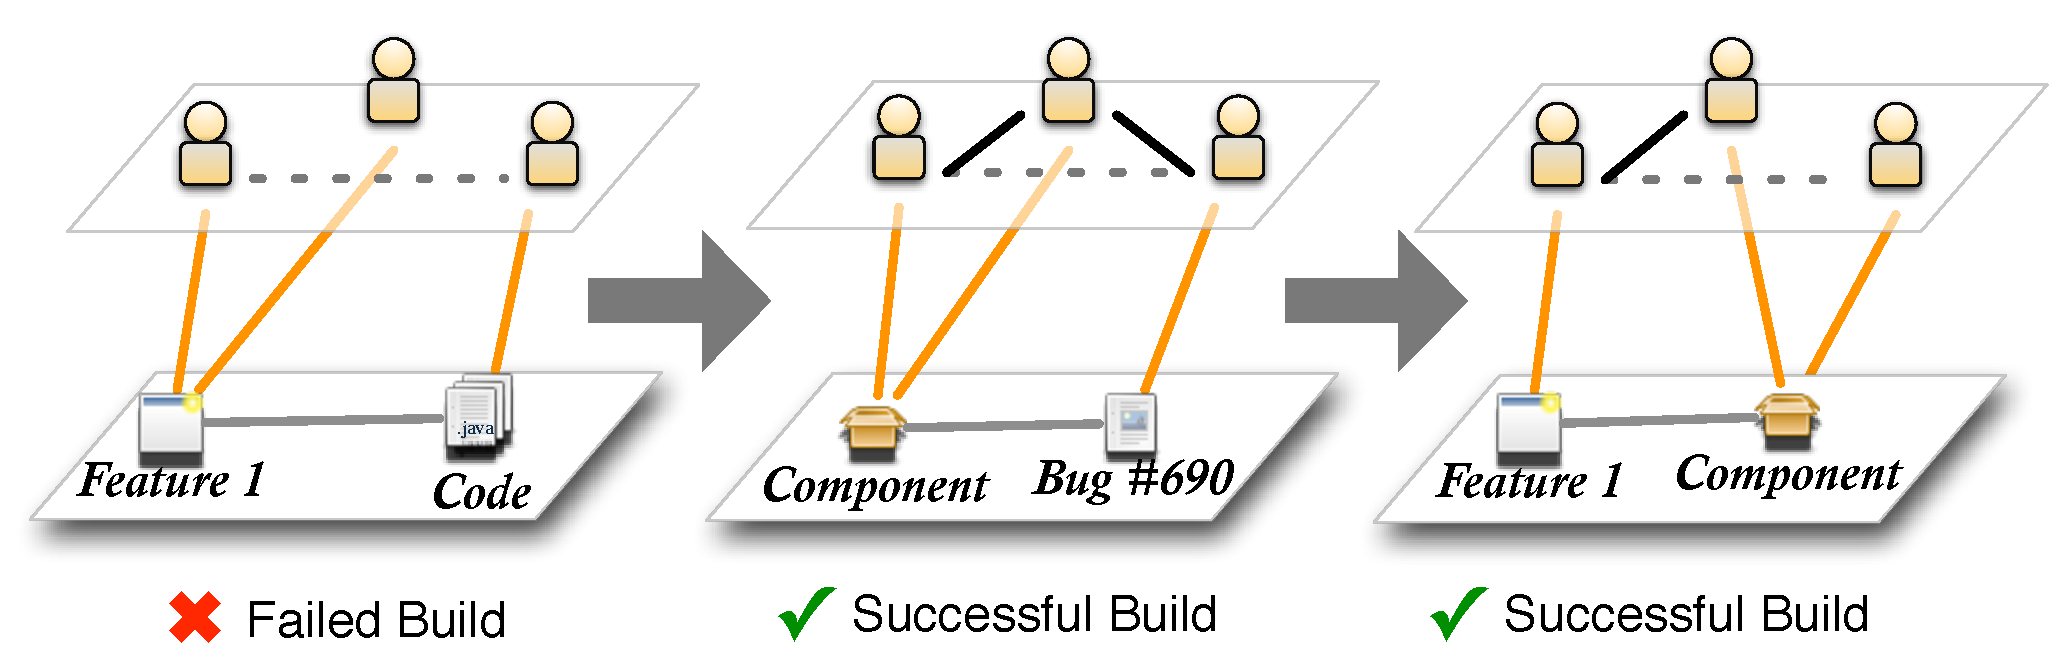
\includegraphics[width=0.9\columnwidth]{figures/bad-to-good}
\caption{Identifying failure inducing coordination gaps.}
\label{fig:multipleplanes}
\end{figure}

\subsection{Our Recommender System}
A recommender system based on socio-technical congruence gaps to prevent a failed build will identify which gaps are most likely to induce build failures. 
Figure~\ref{fig:multipleplanes} shows the social and technical networks for three builds. 
Developers are connected by working on the same artifact and by dependent artifacts. 
We see that the failed build exposes two socio-technical gaps. 
A first glance, this might lead to the conclusion that these gaps are related to build failures. 
Further examination of the two following successful builds suggests that only one gap is bad since the other gap exists in one of the successful builds as well. 
To generate our recommendations we connect people in two ways: (1) on the technical level and (2) at the social level. 

\begin{description}
\item[Technical Level.] 
We mine repositories such as tracking systems and code for technical connections. 
For example, two developers have a technical connection if they work on dependent components or related bug fixes.
\item[Social Level.]
Social level connections can be found by mining email, chat, or comments~\cite{cataldo:cscw:2006}. 
In particular we need to focus on the tasks that are represented by the mined technical connections. 
\end{description}

We could draw data from repository system by IBM called Jazz, which stores issue tracking, source code, and change sets in a single database. 
Jazz records associations between work items and change sets, as well as the results of integration builds. 
A build, therefore, includes the code contributions between the current integration build and the previous integration build. 
Thus, we can identify who has contributed to each integration build and who has coordinated about change sets that were included in a particular build.

We also draw data from open-source projects. 
In an open-source project that does not use Jazz, we can identify change sets from their source code repositories, and corresponding tracker items or development mailing list items based on commit logs. 
Prior to the data mining, the project's development system must be studied and understood in order to provide good recommendations.

\section{A Course on Globally Distributed Software Development}
To answer our final research question for this thesis \textbf{RQ 2.4:} \emph{Can recommendations be given in a timely manner?} we conduct a case study together with students taking a class in globally distributed software development.
The reasoning for choosing this student course as the basis for exploring our final research question has several reasons:
\begin{itemize}
\item Providing a project infrastructure that supports data collection.
\item The distribution of the course across countries ensures a minimum at electronically recordable and mineable communication data being generated.
\item A course setting allows for more control to ensure data quality.
\item A course setting enables better access to interviews and discussions with the study participants.
\end{itemize}

%Providing a project infrastructure that supports data collection.
%The distribution of the course across countries ensures a minimum at electronically recordable and mineable communication data being generated.
%A course setting allows for more control to ensure data quality.
%A course setting enables better access to interviews and discussions with the study participants.
%lead into next section

\section{Setting}
\section{Background and Related Work}
\section{Methodology}
\section{Findings}
\section{Discussion}
\section{Conclusions}
